\documentclass[12pt]{extarticle}
\usepackage[utf8]{inputenc}
\usepackage{cite}
\usepackage{graphicx}
\usepackage[export]{adjustbox}
\usepackage{amsfonts}
\usepackage{amsmath}


\usepackage{algorithm}
\usepackage[noend]{algpseudocode}
\usepackage{subfigure}
\graphicspath{ {./images/} }

\title{Technical Report}
\author{Yasin Yıldırım}
\date{July 2019}

\begin{document}

\maketitle

\section{Introduction}
\subsection{Problem definition}
For an histogram of an image like the given in Fig.\ref{fig:img1-a}, the problem is to find the dominant peaks within the histogram as shown in Fig.\ref{fig:img1-b}. Dominant peaks can be mixed with noise depending on input image and its important for a proposed method to be able to identify the dominant peaks in a robust and stable fashion.

\begin{figure}
\centering     %%% not \center
\subfigure[ Input image]{\label{fig:img1-a}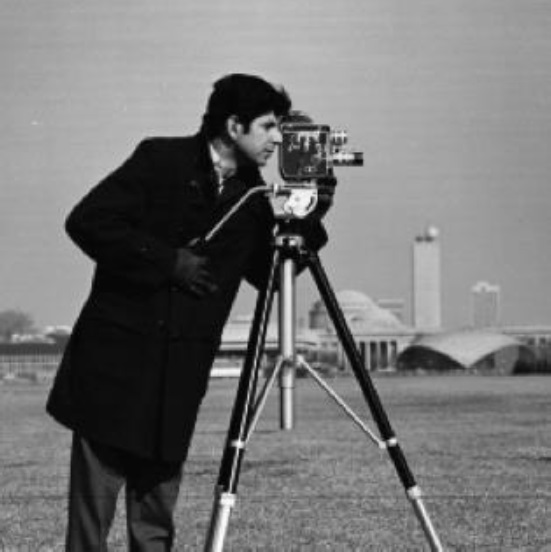
\includegraphics[width=30mm]{img-1}}
\hspace{0.5mm}
\subfigure[Histogram and found dominant peaks]{\label{fig:img1-b}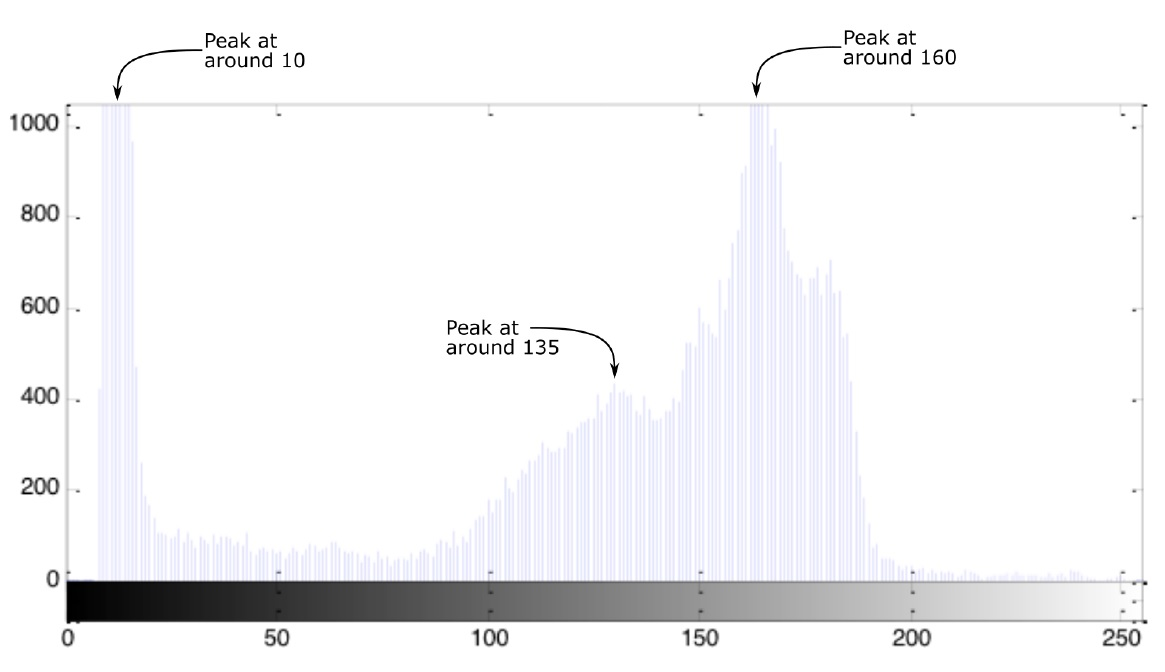
\includegraphics[width=60mm]{hist-1}}
\caption{Input image and its histogram: 3 dominant peaks are pointed as a desired output.}
 \label{fig:img1}
\end{figure}

\subsection{Related approaches as a solution}
There are different potential solutions to the given problem, for instance \textbf{k-means} clustering or modelling components as \textbf{Gaussian Mixture Models} (GMM). One down side of these approaches is that we have to choose number of components, $k$, correctly. It is not possible to form an online dominant peak detection algorithm works on real-time by choosing $k$ manually. There are methods for choosing $k$ such as using Silhouette score, but they require extra computational cost for finding optimal k.

\textbf{GMM} and \textbf{k-means} are based on random initialization which makes the solution non-deterministic \cite{duda2012pattern}, \cite{bishop2006pattern}. Best practice for initialization of GMM, with the Expectation-Maximization algorithm for instance, requires running of the algorithm with multiple random initialization and choosing the stable one as a final initialization. This also leads to extra computational cost. 

\section{Algorithm}

\subsection{High level and intuitive explanation}
Evaluating a histogram as a discrete valued one dimensional signal, we can devise an algorithm by considering the 1D signal as a topological map similar to the watershed algorithm. Starting from the highest level of the histogram values to zero, each point visited in decreasing order and new peaks are created or the current point assigned to left or right neighbour's existing component depending on whether the left or right neighbours are already visited or not. As an analogy, consider a water level in its maximum and it is decreasing in unit degree. Each time currently visited point constitutes a peak of an island whenever the water level reaches a local maximum. Two islands merge together whenever it reaches a local minimum, and higher island is assigned as a parent of lower island in their union. More formal explanation of this approach in terms of computational topology is given in Section \ref{math_background}.
\subsection{Mathematical background} \label{math_background}
\textbf{Persistent homology} is an algebraic method for identifying topological structures such as components, clusters or holes of data \cite{edelsbrunner2010computational}. Formally, let $ u_0, u_1,..., u_k $ be points in $ \mathbb{R}^d $ and \textit{affine combination} of the $u_i$ for a point $x$ is defined as $x = \sum_{k}^{i=0} \lambda_i u_i \impliedby  \sum_{k}^{i=0}\lambda_i = 1 $.
Set of affine combinations forms the \textit{affine hull}. If all $\lambda_i$ are nonnegative then affine combination is a convex combination. The set of convex combinations is called as \textit{convex hull}.

\textbf{Simplicial complexes:} The k+1 points are affinely independent if any two affine combinations satisfies :
$ x = \sum \lambda_i u_i$ and $y = \sum \mu_i u_i,$
are the same $\iff \lambda_i = u_i $ for all $i$.
Convex hull of k+1 affinely independent points, $\sigma=conv\{ u_0, u_1,...,u_k  \} $, forms a \textit{k-simplex} whose dimension is k. First three dimensional simplices, 0-simplex, 1-simplex and 2-simplex, have special names of \textit{vertex}, \textit{edge} and \textit{triangle}, respectively. Sets of simplices having proper intersections meaning that two simplices of K are either disjoint or intersect in a common face and that are closed under taking faces are called \textit{simplicial complexes} \cite{edelsbrunner2010computational}. 

\textbf{Persistent homology:} Let K be a simplicial complex.
A nested sequence of subsets that starts with the empty complex and ends with the complete complex forms the filtration of K as given in equation \eqref{equation1}:
\begin{equation}\label{equation1}
\emptyset= K_0 \subseteq K_1 \subseteq\cdots\subseteq K_n = K.
\end{equation}
For a homology class $c$ born at $K_i$ and died in $K_j$, the persistence of $c$ is $j-i$ \cite{edelsbrunner2010computational}, \cite{edelsbrunner2008persistent}. 

\subsection{Selecting dominant peaks with outlier detection}
 Number of dominant peak points is very small in comparison to total histogram length. For instance, natural images mostly contains a few dominant peaks compared to histogram length which equals to 256 for a grayscale 8-bit image. Thus, it is possible to consider dominant peaks as an outliers within the all \textbf{barcodes} found with the persistent topology of a histogram. Outliers are observations that deviate significantly from other observations of the distribution. It is easy to perform outlier detection when assuming that the regular data come from a known distribution, since outliers won't fit the known mathematical model of the data. In our case, most of the barcode values are within the low range and they lay on a linear model like a fitted line with fixed margin. However, dominant peaks have much higher barcode values in which they don't fit the other observations, like outliers. The example histogram and found barcodes are shown in \ref{fig:img1}, in which barcode values are displayed with red points and weak barcode values are colored blue.
 \begin{figure}
\centering     %%% not \center
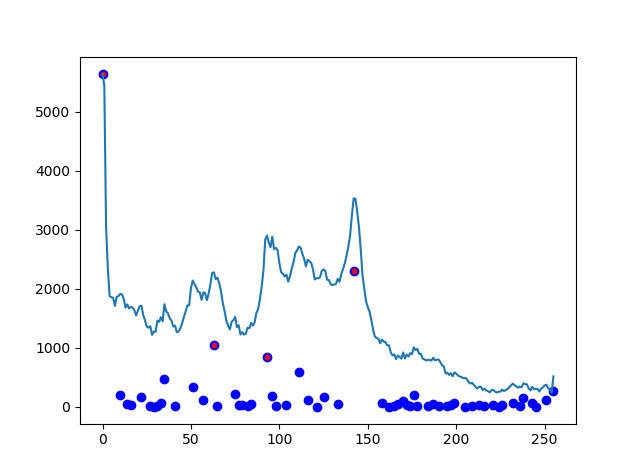
\includegraphics[width=90mm]{Figure_2.png}
\caption{ Red channel histogram of a sample image: Accepted dominant peaks are shown as red points wheres the rejected peak candidates are shown as blue points.}
 \label{fig:img2}
\end{figure}

 The median is a robust statistic that it is not influenced by outliers. \textbf{Median Absolute Deviation} (MAD) is used in order to detect outliers. Formally, for each barcode values $b_i$, distance to the median is calculated and MAD is chosen from the median of these deviations, as shown in equation \eqref{equation2}:
 
 \begin{equation}\label{equation2}
     MAD = median\{ \left | b_i - \tilde{b}  \right | \} 
 \end{equation}

where $\tilde{b}$ denotes median of the barcodes. Then, MAD based z-scores are calculated for each barcode as in the equation \eqref{equation3}:

 \begin{equation}\label{equation3}
     m_i = k* \frac{ \left | b_i - \tilde{b}  \right | }{MAD}
 \end{equation}
 
where $m_i$, $k$ are the MAD based z-score of barcode $b_i$ and quartile coefficient respectively. Finally, dominant peaks are chosen such that only the peaks with the certain z-scores that are higher than the cut-off values are accepted. Formally, each barcode $b_i$ is accepted as peak $p_i$ if $ m_i > T $, for the given cut-off threshold $T$.

\section{Implementation}
Implementation is done in C++ language. \textit{Libbmp} library \cite{dickmannbitmap} is used for input and output operations in bitmap files, which is used in the driver program (\textit{main.cpp}). CMake is used as a build tool in the project.
\subsection{Building the project}
\textbf{Requirements:} Project is built and tested on Windows with MSVC++ compiler with c++17 language standard enabled. A C++ compiler with minimum c++11 features is required to build the project. CMake is required in order to build the project seamlessly. Since the project is tiny, it is also possible to easily build the project manually using compiler commands such as gcc and clang.
\begin{verbatim}
cd hist-peaks
mkdir build
cd build
cmake ..
\end{verbatim}
For Windows, it generates Visual Studio solution file and it can be directly built and run from Visual Studio. For Linux or MacOS, project can be built with \textit{Make} by typing the following command inside build directory:
\begin{verbatim}
make
\end{verbatim}
\subsection{Running the project}
\textit{hist-peaks.exe} executable file should be generated after building the project (Tested on Windows only). The driver program accepts bitmap file path as an input. In order to run the program type the following:
\begin{verbatim}
hist-peaks.exe <input-bitmap-file>
\end{verbatim}
 If no input file is provided, the default image path, which is \textit{'data/test1.bmp'}, is used.
 
\bibliographystyle{ieeetr}
\bibliography{M335}

\end{document}
